\def\mytitle{ASSIGNMENT-1}
\def\myauthor{Maringanti Vaibhava Praneeth}
\def\contact{vaibhavapraneeth@gmail.com}
\def\mymodule{Future Wireless Communications (FWC)}
\documentclass[10pt, a4paper]{article}
\usepackage[a4paper,outer=1.5cm,inner=1.5cm,top=1.75cm,bottom=1.5cm]{geometry}
\twocolumn
\usepackage{graphicx}
\graphicspath{{./images/}}
\usepackage[colorlinks,linkcolor={black},citecolor={blue!80!black},urlcolor={blue!80!black}]{hyperref}
\usepackage[parfill]{parskip}
\usepackage{lmodern}
\usepackage{tikz}
\usetikzlibrary{arrows,shapes.gates.logic.US,shapes.gates.logic.IEC,calc}
\usepackage{karnaugh-map}

\usepackage{tabularx}
%\documentclass{article}
%\documentclass[tikz, border=2mm]{standalone}
%\usepackage{tikz}
%\usepackage{circuitikz}
\usetikzlibrary{calc}

\renewcommand*\familydefault{\sfdefault}
\usepackage{watermark}
\usepackage{lipsum}
\usepackage{xcolor}
\usepackage{listings}
\usepackage{float}
\usepackage{titlesec}

\titlespacing{\subsection}{1pt}{\parskip}{3pt}
\titlespacing{\subsubsection}{0pt}{\parskip}{-\parskip}
\titlespacing{\paragraph}{0pt}{\parskip}{\parskip}
\newcommand{\figuremacro}[5]{
    \begin{figure}[#1]
        \centering
        \includegraphics[width=#5\columnwidth]{#2}
        \caption[#3]{\textbf{#3}#4}
        \label{fig:#2}
    \end{figure}
}

\lstset{
frame=single, 
breaklines=true,
columns=fullflexible
}

%\thiswatermark{\centering \put(400,-128.0){\includegraphics[scale=0.3]{logo}} }
\title{\mytitle}
\author{\myauthor\hspace{1em}\\\contact\\IITH\hspace{0.5em}-\hspace{0.6em}\mymodule}
\date{22-12-2022}
\begin{document}
  \maketitle
  \tableofcontents
  \begin{abstract}
      This manual explains about a logic circiut by taking two inputs A=WX and B=YZ so we comapring these two inputs and if A>B then the function F=1 if not F=0 so for that we are deriving minimized sum of product for F:
%\figuremacro{h}{diag}{}{}{0.9}
  \end{abstract}


  \section{Components}
  \begin{tabularx}{0.4\textwidth} { 
  | >{\centering\arraybackslash}X 
  | >{\centering\arraybackslash}X 
  | >{\centering\arraybackslash}X
  | >{\centering\arraybackslash}X | }
\hline
 \textbf{Component}& \textbf{Values} & \textbf{Quantity}\\
\hline
Arduino & UNO & 1 \\  
\hline
JumperWires& M-M & 10 \\ 
\hline
Breadboard &  & 1 \\
\hline
LED & &1 \\
\hline
Resistor &220ohms & 1\\
\hline
\end{tabularx}



\begin{center}
Figure.a
\end{center}

\section{Truth Table}
  \begin{tabularx}{0.46\textwidth} { 
  | >{\centering\arraybackslash}X 
  | >{\centering\arraybackslash}X 
  | >{\centering\arraybackslash}X
  | >{\centering\arraybackslash}X 
  | >{\centering\arraybackslash}X 
  | >{\centering\arraybackslash}X 
  | >{\centering\arraybackslash}X 
  | >{\centering\arraybackslash}X 
  | >{\centering\arraybackslash}X 
  | >{\centering\arraybackslash}X | }


\hline
\textbf{W} & \textbf{X} & \textbf{Y} & \textbf{Z}\ & \textbf{F}\\
\hline
0 & 0 & 0 & 0 & 0 \\  
\hline
0 & 0 & 0 & 1 & 0 \\ 
\hline
0 & 0 & 1 & 0 & 0 \\
\hline
0 & 0 & 1 & 1 & 0 \\
\hline
0 & 1 & 0 & 0 & 1 \\  
\hline
0 & 1 & 0 & 1 & 0 \\ 
\hline
0 & 1 & 1 & 0 & 0 \\
\hline
0 & 1 & 1 & 1 & 0 \\
\hline
1 & 0 & 0 & 0 & 1 \\
\hline
1 & 0 & 0 & 1 & 1 \\
\hline
1 & 0 & 1 & 0 & 0 \\
\hline
1 & 0 & 1 & 1 & 0 \\
\hline
1 & 1 & 0 & 0 & 1 \\
\hline
1 & 1 & 0 & 1 & 1 \\
\hline
1 & 1 & 1 & 0 & 1 \\
\hline
1 & 1 & 1 & 1 & 0 \\
\hline
\end{tabularx}
\begin{center}
 Truth table Boolean Function "F"
\end{center}

\section{K-map Implementation}


    \begin{karnaugh-map}
        \manualterms{0,0,0,0,1,0,0,0,1,1,0,0,1,1,1,0}
        \implicant{4}{12}
        \implicant{12}{9}
        \implicantedge{12}{12}{14}{14}
    \end{karnaugh-map}

    

\begin{center}
Figure.a
\end{center}
  

 \paragraph {Reducing the boolean Function}:\\
    F=wxy'z'+wxy'z+wxy'z'+w'xy'z'+wxy'z'+wxy'z+wx'y'z'+wx'y'z\\
    F=wxy'(z+z') + xy'z'(w+w')+ wxy'(z+z')+wx'y'(z+z')\\
    F=wxy'+xy'z'+wy'(x+x')\\
 Reduced expression using K-maps is\\
 F=wxy'+xy'z'+wy'\\
 
\section{logical Diagram}




  \thispagestyle{empty}
  \tikzstyle{branch}=[fill,shape=circle,minimum size=3pt,inner sep=0pt]
  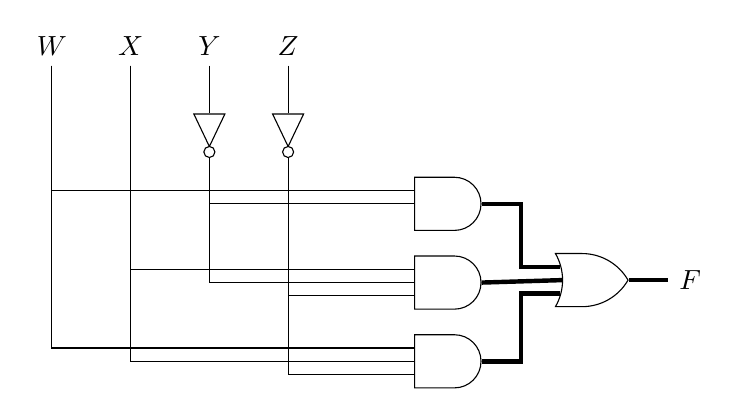
\begin{tikzpicture}[label distance=2mm]

\node (w) at (0,0) {$W$};
\node (x) at (1,0) {$X$};
\node (y) at (2,0) {$Y$};
\node (z) at (3,0) {$Z$};

\node[not gate US, draw, rotate=-90] at ($(y)+(0,-1)$) (Not2) {};
\node[not gate US, draw, rotate=-90] at ($(z)+(0,-1)$) (Not1) {};
\node[and gate US, draw, logic gate inputs=nnn, font=\bfseries\color{red}] at ($(y)+(3,-2)$) (and1) {};
\node[and gate US, draw, logic gate inputs=nnn, font=\bfseries\color{red}] at ($(and1)+(0,-1)$) (and2) {};
\node[and gate US, draw, logic gate inputs=nnn, font=\bfseries\color{red}] at ($(and2)+(0,-1)$) (and3) {};
\node[or gate US, draw, logic gate inputs=nnn, anchor=input 1] at ($(and1.output -| and2.output -| and3.output)+(1,-.8)$) (or) {};

\draw (w) |- (and1.input 1);
\draw (w) |- (and3.input 1);

\draw (x) |- (and2.input 1);
\draw (x) |- (and3.input 2);

\draw (y) |- (Not2.input);
\draw (z) |- (Not1.input);

\draw (Not2.output) |- (and1.input 2);
\draw (Not2.output) |- (and2.input 2);

\draw (Not1.output) |- (and2.input 3);
\draw (Not1.output) |- (and3.input 3);


\draw [ ultra thick] (and1.output) -- ++(0.5cm,0) |- (or.input 1) 
        node [shift={(-0.65em,0.75ex)}, font=\tiny] {};
\draw [ ultra thick] (and2.output) -- (or.input 2) 
        node [shift={(0.65em,0ex)}, , font=\tiny] {};
\draw [ ultra thick] (and3.output) -- ++(0.5cm,0) |- (or.input 3) 
        node [shift={(-0.66em,-0.75ex)}, , font=\tiny] {};

\draw [, ultra thick] (or.east) -- ++(0.5cm,0) node [right] {$F$};


\end{tikzpicture}

    
\section{Implementation}
  \begin{tabularx}{0.46\textwidth} { 
  | >{\centering\arraybackslash}X 
  | >{\centering\arraybackslash}X 
  | >{\centering\arraybackslash}X
  | >{\centering\arraybackslash}X 
  | >{\centering\arraybackslash}X 
  | >{\centering\arraybackslash}X 
  | >{\centering\arraybackslash}X 
  | >{\centering\arraybackslash}X 
  | >{\centering\arraybackslash}X
  | >{\centering\arraybackslash}X
  | >{\centering\arraybackslash}X
  | >{\centering\arraybackslash}X
  | >{\centering\arraybackslash}X
  | >{\centering\arraybackslash}X
  | >{\centering\arraybackslash}X 
  | >{\centering\arraybackslash}X | }


\hline
\textbf{Arduino PIN} & \textbf{INPUT} & \textbf{OUTPUT} \\ 
\hline
\textbf 2 & W & \\
\hline
\textbf 3 & X & \\
\hline
\textbf 4 & Y & \\
\hline
\textbf 5 & Z & \\
\hline
\textbf 8 & & F \\
\hline
\end{tabularx}

\begin{center}
    Connections
\end{center}

    \paragraph{Procedure}:\\
    1. Connect the circuit as per the above table.\\
    2. Connect the output pin to LED\\
    3. Connect inputs to Vcc for logic 1, ground for logic 0\\
    4. Execute the circuit using the below code.\\
  
   \begin{tabularx}{0.55\textwidth} { 
  | >{\centering\arraybackslash}X |}
\hline
https://github.com/vaibhavapraneeth/FWC/blob/main/
assignments/ide/src/assign1.cpp\\
\hline
\end{tabularx}

   \paragraph{Problem-2}:\\
1. Change the values of W,X,Y,Z in the code and verify the Truth Table\\


\bibliographystyle{ieeetr}
\end{document}